\documentclass[12pt]{article}
\usepackage[margin=1in]{geometry}
\usepackage{graphicx}
\usepackage{amsmath}
\usepackage{float}
\usepackage{hyperref}

\title{Politician in the Media}
\author{Team Name Here}
\date{\today}

\begin{document}

\maketitle

\section{Introduction}
Provide an overview of your project and summarize the key findings.

\section{Data}
Describe the dataset, including the number of articles, sources, and any filtering or sampling decisions.

\section{Methods}
Explain the methodology used for topic and sentiment analysis.

\section{Results}
Present your findings, including topic characterizations and sentiment distributions.

\begin{figure}[H]
    \centering
    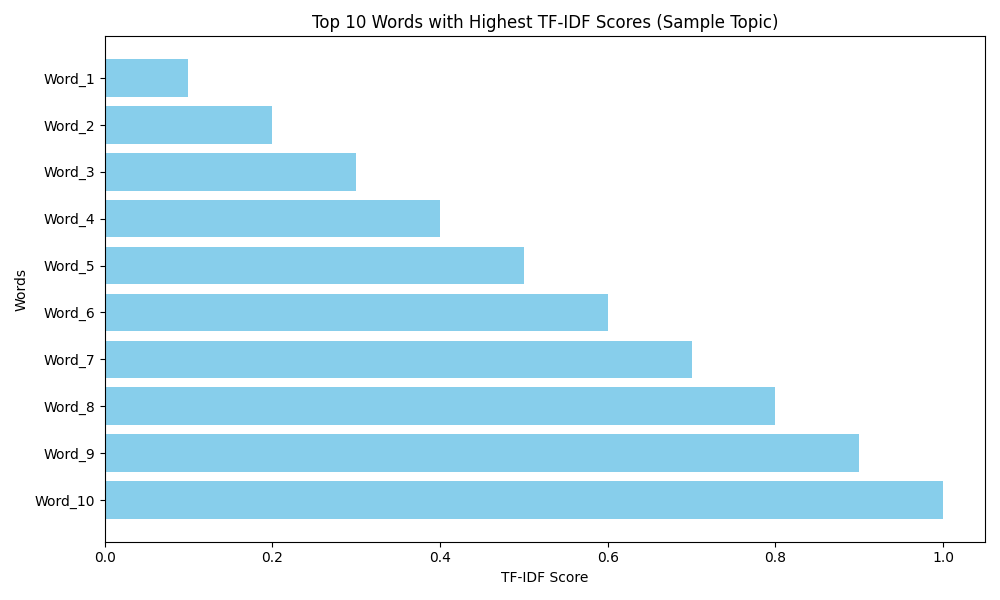
\includegraphics[width=0.8\textwidth]{./figures/top_tfidf_words.png}
    \caption{Top 10 words with the highest TF-IDF scores per topic.}
    \label{fig:tfidf}
\end{figure}

\section{Discussion}
Interpret the results and discuss their implications.

\section{Group Member Contributions}
Detail the contributions of each group member.

\section{References}
Include references here in AAAI format.

\end{document}
